%!TEX root = ../../thesis.tex

\section{Background}

  \subsection{Behaviour of Liquid}
    This thesis is concerned with the behaviour of liquid at the atomic scale.
    At the macro scale, the behaviour of liquid is simple and calculable.
    Modern computers can simulate the movement of liquids using the Navier-Stokes equations with accuracy and speed.
    This does not hold true when modelling fluid at the scale of individual atoms and molecules, where the behaviour is determined purely by electrical interactions.
    These interactions are chaotic and therefore simulation of any reasonable sized volume demands prohibitive computing resources.

    Water is a liquid comprised of the molecule $H_{2}O$.
    This molecule is polar, meaning one side has a net positive charge and the other has a net negative charge.
    This simple fact is responsible for very complex behaviour when dealing with a liquid body of any reasonable size.

    \begin{figure}
        \begin{center}
            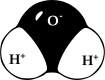
\includegraphics{content/introduction/graphics/polarWater}
        \end{center}
        \caption{A single polar water molecule}
        \label{fig:waterMolecule}
    \end{figure}

    The unifying theme of this thesis is the interactions that take place at the boundary between liquids and solids.
    Interactions of interest occur on the liquid side of the boundary.
    Of particular interest what happens directly at the boundary, within a layer titled the double layer.

    The electric field of the solid's interior would be affected by the accumulation of charge at its surface, but this should not affect the analysis of the exterior layer.
    It is important to note that a solid in the context of this thesis is not simply the walls of a container, but may also refer to solid particles, even molecules, within a liquid.
    This is the case for emulsified substances such as paints where the formed double layer determines the stability of the emulsion.

    This thesis focusses on two applications of interfacial double layers with respect to electrical engineering. Firstly, it looks at a method of harvesting power from water by way of a mechanism that has no moving parts; and secondly, it models the electrical impedance that is seen by a medical implant when placed inside a biological system. The second application is where the majority of the research effort can be found.

    \subsection{Molecular Simulation}
    Physical simulations involving the properties of materials and interactions with radio-waves are a common tool for any RF engineer. There are many areas in science and engineering that benefit from powerful computer simulation. Many modern-day computer games simulate the position and velocity of thousands of objects, such as bullets and buildings breaking apart, in near real-time.

    These kinds of simulations generally involve calculating the state of a system of objects at a specific time, then adjusting the all of the parameters based the physics of that system at a specific time, and repeating this process for as long as the simulation need continue.

    Finite-difference time-domain (FDTD) simulation is a common technique for calculating electrical fields and resulting currents and voltages in the field of electrical engineering. Such simulations can involve hundreds of thousands, \emph{sometimes millions}, of objects. Generally these objects are elements of a 3D mesh that has been created to represent the geometry of the system to be simulated. In such a simulation, each mesh element at every time step needs its various parameters (e.g. temperature, electromagnetic fields, electrical current and voltage) to be calculated based on the parameters of neighbouring objects in the mesh. Because of the dependence on neighbouring parameter values, each time-step may take many passes over each element in a system to calculate the final state before moving on. These sorts of simulations are extremely valuable for the radio frequency engineer as systems of a practical size can be simulated relatively quickly on modest computing hardware.

    At this point it seems natural to assume that we could model the behaviour of atoms and molecules in a liquid. Doing this would allow simulation of the interactions that take place at the fluid-soild boundary. It is possible to run such molecular dynamics (MD) simulations, however the number of atoms and molecules in any practical sized volume of fluid is astronomical.

    The molar mass of water is defined as $18.0528\thinspace g/Mol$, which represents the amount of water in moles per gram. One gram of water is defined as one millilitre so we can say that for every millilitre of water we have we have an eighteenth of a mole of water. Avagadro's constant, the number of constituent particles per mole of a given substance, is $6.0221\thinspace \times 10^{23}$. Therefore we have one eighteenth of Avagadro's constant in water molecules, which is about $3.3333\times 10^{22}$ molecules. That is 33 333 333 333 333 333 333 333 molecules! The behaviour of double layers in the applications of this research require a far greater volume than $1\thinspace ml$ to be useful, putting molecular simulation out of the picture for the applications discussed in this thesis for the foreseeable future.

  \subsection{Interfacial Double Layer}

    \begin{figure}
      \begin{center}
        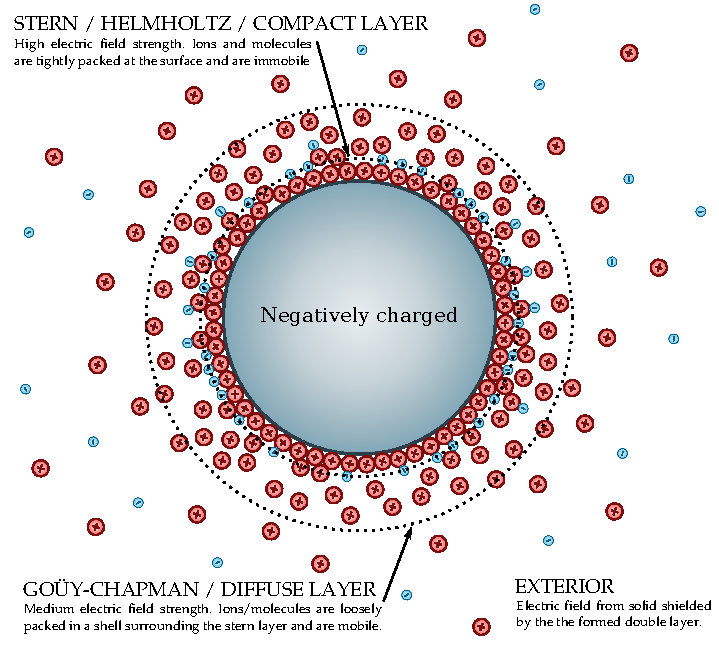
\includegraphics{content/introduction/graphics/doubleLayer_labelled.pdf}
      \end{center}
      \caption{Anatomy of the double layer}
      \label{fig:doubleLayer_anatomy}
    \end{figure}

    Double layers appear to varying degrees almost everywhere an electrolytic fluid and a solid are in contact. They are very small {Todo: quantify typical double layer sizes}, existing in the micro scale, and are responsible for a number of macro scale effects. Such effects are the stability of emulsions {Todo: find instances where double layers play a role}, the something else and even... They are a natural response when two systems of arrangement are brought to contact - fixed and fluid arrangements of charged particles.

  \subsubsection*{Physical Description}
    Double layer formation is the result of a liquid system responding to an imbalance of charge distribution. Atoms within a solid domain are static, they cannot repel each other or rearrange themselves. In a fluid the opposite is true, each freely moving charged entity will attempt to distance itself from others of like charge and move toward those of opposite charge. When these two domains are brought into contact with one another, the one whose elements are free to move (the liquid), moves to accommodate the imbalance in charge between the two domains. The effect of which is that an electrolytic liquid attracts atoms and molecules with a net opposite charge to the surface of the solid.

  \subsubsection*{Formation}
    {\color{blue}
    In order for a double layer to form, the liquid phase must contain ions, charged molecules, or polar molecules.
    This means there are likely to be non-participating elements within the fluid, that is, elements not affected by the charge {Todo: check affected and effected} of surrounding elements.
    The reverse case is also true {Todo: is this correct?, I just made it up} where an electrolyte solution comes in contact with a electrically neutral and stable solid. Although this case is not as obvious as one may think. For example, placing pure water in a glass flask, it may be assumed, would not cause the formation of a double layer. Glassware in used throughout chemistry laboratories as it reacts with very little and pure water with no salt ions should be fairly stable. This is not the case however as glass in contact with water undergoes a process of deprotonation at the boundary. This deprotonation is where $H^{+}$ ions are torn from the surface of the glass and enter the liquid phase. As this happens, the surface of the glass is left negatively charged. Subsequently, a double layer is formed from polar water molecules and hydrated protons.
    }



    Figures \ref{fig:doubleLayer_set1} and \ref{fig:doubleLayer_set2} illustrate the formation of such a layer around a charged object that, for the sake of illustration, instantaneously appears in a settled electrolyte solution. In these figures, the spacing of depicted fluid elements do not represent the density of a liquid system and the smooth surface of the charged object in no way resembles the surface of a solid at the scale of individual atoms.

    The first set of images, figure \ref{fig:doubleLayer_set1}, depict charged elements in the fluid responding to the presence of the solid by aligning themselves with the induced field and migrating toward or away from the object. The second set of images, figure \ref{fig:doubleLayer_set2}, shows continued migration of charged particles and the formation of the Stern layer at the solid-liquid interface. Members of this layer are bound so strongly to the object that they are effectively immobile, i.e., they are adsorbed to the solid object. A substantial proportion of the initial electrical field from the solid is shielded by the Stern layer.

    Outside the Stern layer, as the field strength continues to diminish with increasing radial distance, ions and molecules are attracted with decreasing strength. This reduction in attraction forms a layer that is thicker than the stern layer and mobile; the ions are free to move locally within this secondary layer. This secondary layer is called the diffuse layer and it is convenient to visualise it as a fluffy cloud of charged particles attracted to, but not trapped upon, the thin Stern layer immediately adjacent to the surface.

    \begin{figure}
      \begin{center}
        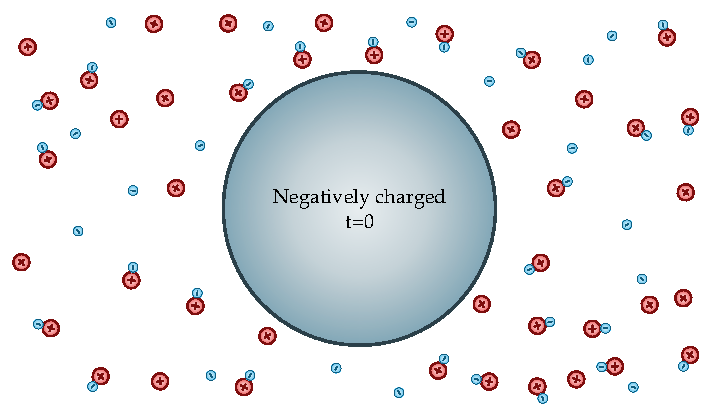
\includegraphics{content/introduction/graphics/doubleLayer_t0.pdf}
        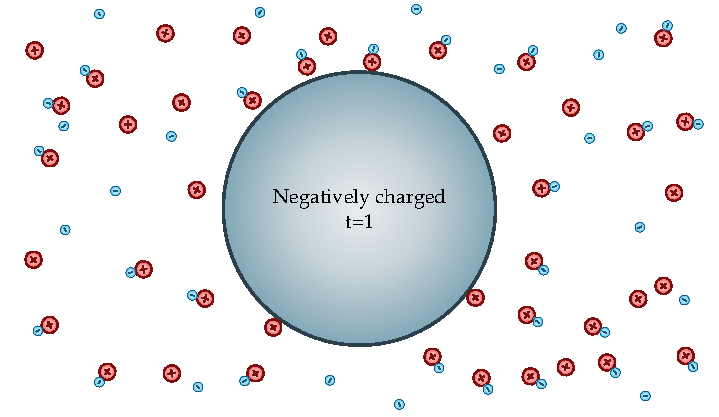
\includegraphics{content/introduction/graphics/doubleLayer_t1.pdf}
        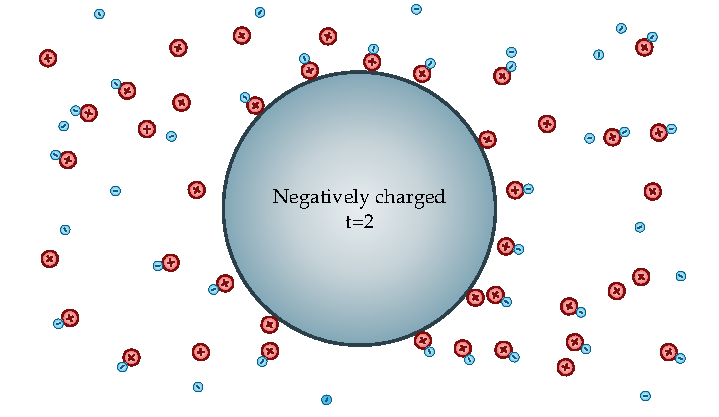
\includegraphics{content/introduction/graphics/doubleLayer_t2.pdf}
      \end{center}
      \caption{Creation of a double layer (time 0-2)}
      \label{fig:doubleLayer_set1}
    \end{figure}

    \begin{figure}
      \begin{center}
        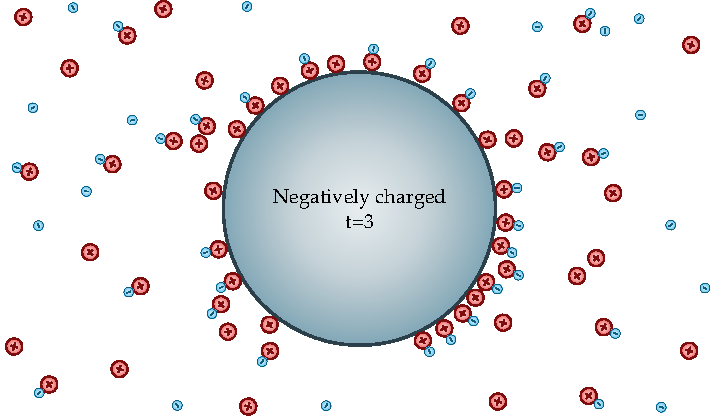
\includegraphics{content/introduction/graphics/doubleLayer_t3.pdf}
        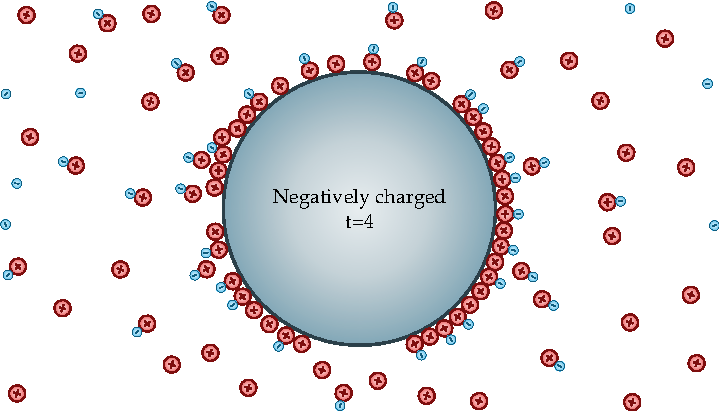
\includegraphics{content/introduction/graphics/doubleLayer_t4.pdf}
        %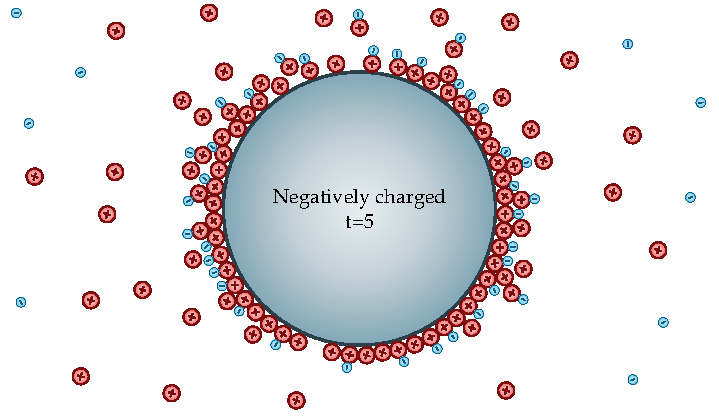
\includegraphics{content/introduction/graphics/doubleLayer_t5.pdf}
        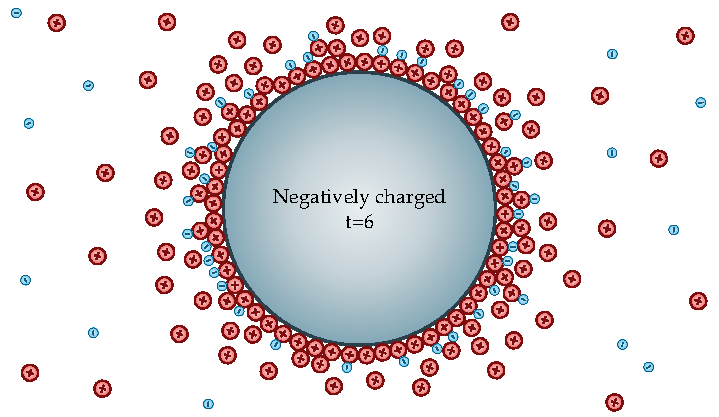
\includegraphics{content/introduction/graphics/doubleLayer_t6.pdf}
      \end{center}
      \caption{Creation of a double layer (time 3-6)}
      \label{fig:doubleLayer_set2}
    \end{figure}


  \subsubsection*{Electrical Behaviour}

\section{Motivation}
  This thesis begins with the question: is it possible to harvest enough electrical energy from flowing water, without moving parts, to power a smart meter?
  The logic being that a harvester without moving parts would last longer than its mechanical equivalents.
  I started by investigating an assortment of possible mechanisms (discussed in detail in Chapter

  I started by investigating
  \begin{itemize}
    \item piezoelectric vibrators,
    \item electrostatic generators, and
    \item streaming potential cells
  \end{itemize}
  as potential harvesting mechanisims.

  The piezoelectric vibrator was the equivalent of a water whistle with a vibrational energy harvester attached.
  The electrostatic generator was a version of Lord Kelvin's Electrostatic Generator with a harvesting application.
  The streaming potential cell was a mystery.

  We knew geologists used streaming potentials to measure underground water flow.
  All we knew about the mechanism was that forcing water through something generated a voltage somehow.
  It was learning about that mechanism and answering the following questions that started me on what became this thesis.
  \begin{enumerate}
    \item Where does the streaming voltage come from?
    \item What role does the geometry of the device play?
    \item Could you change the materials to get more voltage?
  \end{enumerate}
  I eventually concluded that streaming cell harvesters were not practical for our application.
  By this time I had a working knowledge of interfacial double layers and their properties.

  My supervisor, Jonathan Scott, was on a sabbatical at Saluda Medical working with implant electrodes.
  There he developed an electrical model of the impedance presented by electrodes immersed in a solution of saline.
  This model would predict the electrical impedance seen between two electrodes when implanted in the spine of a human.
  Most of the behaviour the model reproduced was a result of interfacial double layers.

  Saluda wanted to know how good a substitute saline was for spinal fluid with regards to electrical impedance.
  There was no way to know and no way to compare solutions, except for using the new model.
  I took the model and started the next stage of my research; characterising fluids based on the impedance they present to electrodes.
  I was able to leverage my understanding of interfacial double layers and apply it to medical engineering.

\section{Publications}

\section{Thesis Outline}
